\documentclass[11pt,a4paper]{article}
\usepackage[margin=1in]{geometry}
\usepackage{amsmath,amssymb,amsthm}
\usepackage{graphicx}
\usepackage{tikz}
\usetikzlibrary{shapes.geometric, arrows, positioning, calc, decorations.pathreplacing, patterns, fit, backgrounds}
\usepackage{algorithm}
\usepackage{algpseudocode}
\usepackage{booktabs}
\usepackage{multirow}
\usepackage{xcolor}
\usepackage{hyperref}
\usepackage[numbers]{natbib}
\usepackage{tcolorbox}

\definecolor{quantumblue}{RGB}{0,102,204}
\definecolor{classicalred}{RGB}{204,51,51}
\definecolor{hybridgreen}{RGB}{51,153,51}
\definecolor{githubgray}{RGB}{36,41,46}

\title{\textbf{Unified Verification Framework for Fault-Tolerant Quantum Random Sampling:\\Bridging k-Uniform States and Measurement-Based Computation}}

\author{H M Shujaat Zaheer\\
\small Master of Science in Computer Science (AI/ML Specialization)\\
\small University of Sialkot, Pakistan\\
\small \texttt{shujabis@gmail.com}}

\date{PhD Research Proposal --- ETH Zurich\\Supervisor: Prof. Dominik Hangleiter}

\begin{document}
\maketitle

\begin{abstract}
Quantum random sampling offers a promising path toward demonstrating quantum computational advantage, yet verification of sampling experiments remains fundamentally challenging. Recent advances in measurement-based quantum computing (MBQC) enable efficient verification through stabilizer measurements \cite{ringbauer2025verifiable}, while fault-tolerant preparation of k-uniform states provides structured entanglement resources \cite{majidy2025scalable}. This proposal identifies a critical gap: \textbf{no unified framework exists to verify quantum random sampling when the underlying resource states are fault-tolerantly prepared k-uniform states}. We propose to develop such a framework by establishing theoretical connections between k-uniformity verification via stabilizer tableaux and direct fidelity estimation (DFE) protocols for MBQC. Our methodology combines the $\Delta$-approximate k-uniformity criterion with stabilizer group sampling to create verification protocols that scale efficiently while maintaining fault tolerance. This research directly addresses three foundational questions: the computational boundaries between quantum and classical sampling, principles governing quantum advantage in verification tasks, and practical constraints from noise on verifiable quantum speedups. The proposed framework aims to enable verified quantum advantage demonstrations using near-term trapped-ion and neutral-atom platforms with $\mathcal{O}(100)$ qubits.

\vspace{0.5em}
\noindent\textbf{Keywords:} Quantum verification, k-uniform states, measurement-based quantum computing, direct fidelity estimation, fault tolerance, quantum random sampling
\end{abstract}

% GitHub Repository Box
\begin{tcolorbox}[colback=githubgray!5!white, colframe=githubgray, title={\textbf{\large Implementation Repository}}, fonttitle=\bfseries\color{white}]
\textbf{Repository:} \url{https://github.com/hmshujaatzaheer/quantum-verification-framework}

\vspace{0.5em}
\textbf{This repository provides a comprehensive Python implementation of the research proposal:}
\begin{itemize}
    \item \textbf{Stabilizer Tableau Module}: Binary symplectic representation for efficient state manipulation and k-uniformity verification via GF(2) rank computation (Eq.~\ref{eq:kuniform})
    \item \textbf{Direct Fidelity Estimation}: Implementation of DFE protocol (Eq.~\ref{eq:fidelity}) with noise modeling
    \item \textbf{Algorithm 1 Implementation}: Adaptive Stabilizer Sampling exploiting k-uniform structure for reduced variance verification (Algorithm~\ref{alg:adaptive})
    \item \textbf{Hybrid Protocol}: Physical-logical verification scheme following \cite{majidy2025scalable}
    \item \textbf{Circuit Construction}: Surface code, color code, and cluster state preparation circuits
    \item \textbf{Benchmarking Suite}: Complete examples comparing DFE vs XEB sample complexity
\end{itemize}

\vspace{0.3em}
\textbf{Installation:}
\begin{verbatim}
git clone https://github.com/hmshujaatzaheer/quantum-verification-framework
cd quantum-verification-framework && pip install -r requirements.txt
python examples/verification_demo.py
\end{verbatim}
\end{tcolorbox}

\section{Introduction}

Quantum computers promise computational advantages over classical machines for specific problems, with quantum random sampling emerging as a leading candidate for demonstrating this advantage \cite{ringbauer2025verifiable}. The central challenge is verification: how can we efficiently certify that a quantum device genuinely produced samples from the correct probability distribution when classical simulation is intractable?

Recent work by Ringbauer et al. \cite{ringbauer2025verifiable} demonstrated efficiently verifiable quantum random sampling using measurement-based quantum computing on trapped ions. Their key insight is that cluster states---the resource states for MBQC---admit efficient verification through direct fidelity estimation (DFE) using stabilizer measurements. Specifically, for a cluster state $|\psi\rangle$ defined by $N$ stabilizer generators $S_1, \ldots, S_N$, the fidelity can be estimated as:
\begin{equation}
F = \frac{1}{2^N} \sum_{s \in \mathcal{S}} \langle s \rangle_\rho
\label{eq:fidelity}
\end{equation}
where $\mathcal{S} = \langle S_1, \ldots, S_N \rangle$ is the stabilizer group.

Independently, Majidy, Hangleiter, and Gullans \cite{majidy2025scalable} introduced scalable fault-tolerant circuits for preparing encoded k-uniform states, where k-uniformity ensures that every k-qubit subsystem is maximally mixed. Their stabilizer-tableau method determines k-uniformity efficiently:
\begin{equation}
\Delta = 2 - 2^{1-r}, \quad r = 2k - I_A
\label{eq:kuniform}
\end{equation}
where $I_A$ counts independent stabilizers after restricting to subsystem $A$.

\begin{figure}[htbp]
\centering
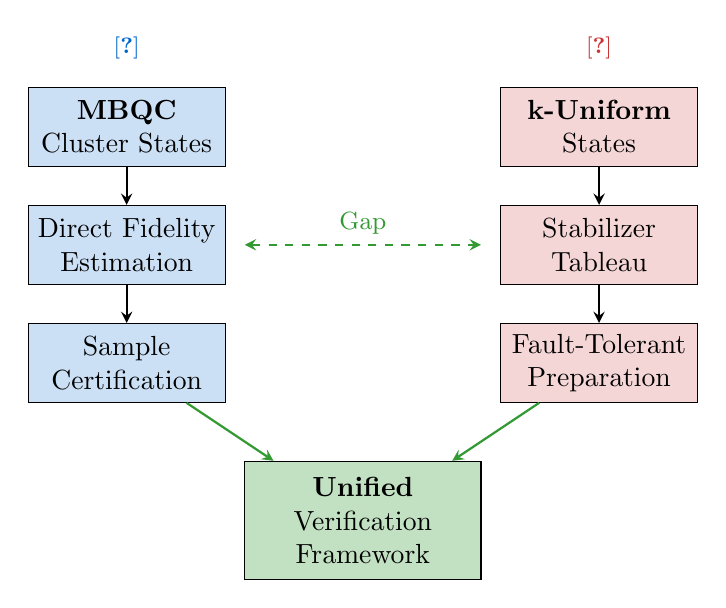
\begin{tikzpicture}[
    block/.style={rectangle, draw, fill=blue!10, minimum width=2.5cm, minimum height=1cm, align=center},
    arrow/.style={->, >=stealth, thick},
    doublearrow/.style={<->, >=stealth, thick, dashed}
]

% Left side - MBQC Verification
\node[block, fill=quantumblue!20] (mbqc) at (0,3) {\textbf{MBQC}\\Cluster States};
\node[block, fill=quantumblue!20] (dfe) at (0,1.5) {Direct Fidelity\\Estimation};
\node[block, fill=quantumblue!20] (verify1) at (0,0) {Sample\\Certification};

% Right side - k-Uniform States
\node[block, fill=classicalred!20] (kunif) at (6,3) {\textbf{k-Uniform}\\States};
\node[block, fill=classicalred!20] (stab) at (6,1.5) {Stabilizer\\Tableau};
\node[block, fill=classicalred!20] (verify2) at (6,0) {Fault-Tolerant\\Preparation};

% Center - Proposed Framework
\node[block, fill=hybridgreen!30, minimum width=3cm, minimum height=1.5cm] (unified) at (3,-2) {\textbf{Unified}\\Verification\\Framework};

% Arrows
\draw[arrow] (mbqc) -- (dfe);
\draw[arrow] (dfe) -- (verify1);
\draw[arrow] (kunif) -- (stab);
\draw[arrow] (stab) -- (verify2);

\draw[doublearrow, color=hybridgreen] (1.5,1.5) -- node[above, font=\small] {Gap} (4.5,1.5);

\draw[arrow, color=hybridgreen, thick] (verify1) -- (unified);
\draw[arrow, color=hybridgreen, thick] (verify2) -- (unified);

% Labels
\node[font=\footnotesize, color=quantumblue] at (0,4) {\cite{ringbauer2025verifiable}};
\node[font=\footnotesize, color=classicalred] at (6,4) {\cite{majidy2025scalable}};

\end{tikzpicture}
\caption{Research gap: Current verification approaches for MBQC and k-uniform state preparation operate independently. This proposal develops a unified framework exploiting the stabilizer structure common to both.}
\label{fig:gap}
\end{figure}

\textbf{Research Gap:} Despite both frameworks relying on stabilizer formalism, no systematic connection exists between k-uniformity verification and MBQC fidelity estimation. Cluster states with specific local rotations may exhibit k-uniform properties for certain subsystems, potentially enabling more efficient verification protocols. Furthermore, the hybrid physical-logical scheme from \cite{majidy2025scalable} has not been analyzed in the context of MBQC verification.

\section{Problem Statement and Existing Work}

\subsection{The Verification Challenge}

Verification of quantum random sampling faces a fundamental tension: any method relying solely on classical samples is inefficient \cite{ringbauer2025verifiable}, requiring exponentially many samples to distinguish quantum from classical distributions. Cross-entropy benchmarking (XEB) \cite{ringbauer2025verifiable} offers practical verification but requires classical simulation of ideal output probabilities---computationally infeasible in the quantum advantage regime.

\subsection{State-of-the-Art Approaches}

\textbf{MBQC Verification \cite{ringbauer2025verifiable}:} Cluster states up to $4 \times 4$ qubits were verified using DFE with root infidelity $\sqrt{1-F}$ bounding total variation distance (TVD):
\begin{equation}
d_{\text{TV}} \leq d_{\text{Tr}} \leq \sqrt{1-F}
\label{eq:bound}
\end{equation}
Qubit recycling enabled sampling from cluster states larger than the physical register via mid-circuit reset \cite{bluvstein2024logical}.

\textbf{k-Uniform State Preparation \cite{majidy2025scalable}:} Transversal circuit architectures achieve fault tolerance while maintaining scalability. For an $[n, \kappa, d]$ code, logical qubits are grouped into $\kappa$-qubit blocks with brickwork-pattern entangling gates. The hybrid physical-logical scheme reduces overhead for arbitrary rotations by selectively unencoding qubits.

\textbf{Fault-Tolerant Operations \cite{bluvstein2024logical, ryananderson2024highfidelity}:} Recent experiments demonstrated logical qubit operations with error rates below physical thresholds using surface codes \cite{acharya2024quantum} and color codes \cite{dasilva2024demonstration}.

\begin{table}[htbp]
\centering
\caption{Comparison of Verification Methods}
\label{tab:comparison}
\begin{tabular}{@{}lccc@{}}
\toprule
\textbf{Method} & \textbf{Sample Efficiency} & \textbf{Computational Efficiency} & \textbf{Fault Tolerance} \\
\midrule
XEB \cite{ringbauer2025verifiable} & $\mathcal{O}(\text{poly})$ & $\mathcal{O}(\exp)$ & No \\
DFE for MBQC \cite{ringbauer2025verifiable} & $\mathcal{O}(\epsilon^{-2})$ & $\mathcal{O}(\text{poly})$ & Partial \\
k-Uniform Tableau \cite{majidy2025scalable} & N/A & $\mathcal{O}(\binom{N}{k})$ & Yes \\
\textbf{Proposed Unified} & $\mathcal{O}(\epsilon^{-2})$ & $\mathcal{O}(\text{poly})$ & \textbf{Yes} \\
\bottomrule
\end{tabular}
\end{table}

\section{Proposed Research}

\subsection{Research Questions}

This proposal addresses three foundational questions identified by Prof. Hangleiter's research program:

\begin{enumerate}
    \item \textbf{Quantum-Classical Boundaries:} What structural properties of k-uniform cluster states determine the classical simulability threshold?
    \item \textbf{Guiding Principles:} Can k-uniformity degree $k$ serve as a sufficient condition for quantum advantage in random sampling verification?
    \item \textbf{Device Constraints:} How does the hybrid physical-logical scheme \cite{majidy2025scalable} affect verification fidelity bounds under realistic noise models?
\end{enumerate}

\subsection{Core Hypothesis}

\textbf{Hypothesis:} For cluster states prepared via fault-tolerant k-uniform circuits, the k-uniformity parameter provides a lower bound on the number of stabilizer measurements required for verification with fixed confidence, enabling adaptive verification protocols that exploit state structure.

\subsection{Proposed Methodology}

\begin{figure}[htbp]
\centering
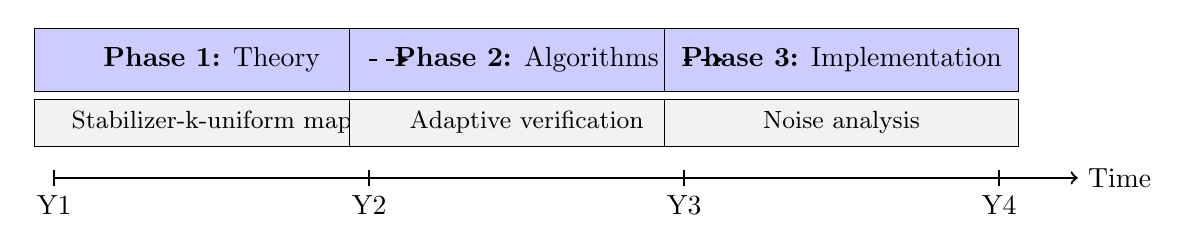
\begin{tikzpicture}[
    phase/.style={rectangle, draw, fill=blue!20, minimum width=4.5cm, minimum height=0.8cm, align=center},
    task/.style={rectangle, draw, fill=gray!10, minimum width=4.5cm, minimum height=0.6cm, align=center, font=\small},
    arrow/.style={->, >=stealth, thick}
]

% Timeline
\draw[thick, ->] (0,0) -- (13,0) node[right] {Time};

% Year markers
\foreach \x/\year in {0/Y1, 4/Y2, 8/Y3, 12/Y4} {
    \draw[thick] (\x,0.1) -- (\x,-0.1) node[below] {\year};
}

% Phase 1
\node[phase] at (2,1.5) {\textbf{Phase 1:} Theory};
\node[task] at (2,0.7) {Stabilizer-k-uniform map};

% Phase 2  
\node[phase] at (6,1.5) {\textbf{Phase 2:} Algorithms};
\node[task] at (6,0.7) {Adaptive verification};

% Phase 3
\node[phase] at (10,1.5) {\textbf{Phase 3:} Implementation};
\node[task] at (10,0.7) {Noise analysis};

% Connections
\draw[arrow, dashed] (4,1.5) -- (4.5,1.5);
\draw[arrow, dashed] (8,1.5) -- (8.5,1.5);

\end{tikzpicture}
\caption{Research timeline with three phases spanning four years.}
\label{fig:timeline}
\end{figure}

\subsubsection{Phase 1: Theoretical Foundation (Year 1-2)}

We will establish the mathematical connection between k-uniformity and DFE sample complexity.

\textbf{Approach:} Extend the stabilizer tableau method from \cite{majidy2025scalable} to cluster states with local rotations $Z(\beta) = e^{-i\beta Z/2}$. For random angles $\beta \in \{0, \frac{\pi}{4}, \ldots, \frac{7\pi}{4}\}$, the stabilizers become:
\begin{equation}
S_k = X_k(\beta_k) \prod_{j \in \mathcal{N}(k)} Z_j
\end{equation}
where $X_k(\beta) = e^{i\beta X_k/2}$ and $\mathcal{N}(k)$ denotes neighbors of site $k$.

\textbf{Key Investigation:} Determine the k-uniformity of random cluster states as a function of lattice dimensions $n \times m$ and rotation angle distribution.

\subsubsection{Phase 2: Algorithm Development (Year 2-3)}

Building on Phase 1, we develop verification algorithms that adapt measurement selection based on k-uniformity structure.

\begin{algorithm}[htbp]
\caption{Adaptive Stabilizer Sampling for Verification}
\label{alg:adaptive}
\begin{algorithmic}[1]
\Require Cluster state $|\psi_\beta\rangle$, target accuracy $\epsilon$, k-uniformity bound $k^*$
\Ensure Fidelity estimate $\hat{F}$ with confidence $1-\delta$
\State Compute stabilizer tableau $T$ for $|\psi_\beta\rangle$
\State Identify k-uniform subsystems via Eq.~\eqref{eq:kuniform}
\State $\mathcal{S}_{\text{priority}} \gets$ stabilizers supported on k-uniform regions
\State $M \gets \lceil 4\epsilon^{-2}\log(2/\delta) \rceil$ \Comment{Sample complexity bound}
\For{$i = 1$ to $M$}
    \If{$i \leq M/2$}
        \State Sample $s_i$ uniformly from $\mathcal{S}_{\text{priority}}$
    \Else
        \State Sample $s_i$ uniformly from full stabilizer group $\mathcal{S}$
    \EndIf
    \State Measure $s_i$ on state preparation, obtain $\sigma_i \in \{+1, -1\}$
\EndFor
\State $\hat{F} \gets \frac{1}{M}\sum_{i=1}^M \sigma_i$
\State \Return $\hat{F}$
\end{algorithmic}
\end{algorithm}

\textbf{Theoretical Justification:} The variance of the fidelity estimator depends on the distribution of stabilizer eigenvalues \cite{ringbauer2025verifiable}:
\begin{equation}
\text{Var}[\hat{F}] = \frac{4}{KM}\mathbb{E}[p_s(1-p_s)] + \frac{4(K-1)}{K}\text{Var}[p_s]
\end{equation}
Prioritizing stabilizers from k-uniform regions reduces $\text{Var}[p_s]$ when noise affects subsystems uniformly.

\subsubsection{Phase 3: Noise Analysis and Implementation (Year 3-4)}

Analyze verification performance under realistic noise models, extending the depolarizing channel analysis from \cite{majidy2025scalable} to the MBQC setting.

\begin{figure}[htbp]
\centering
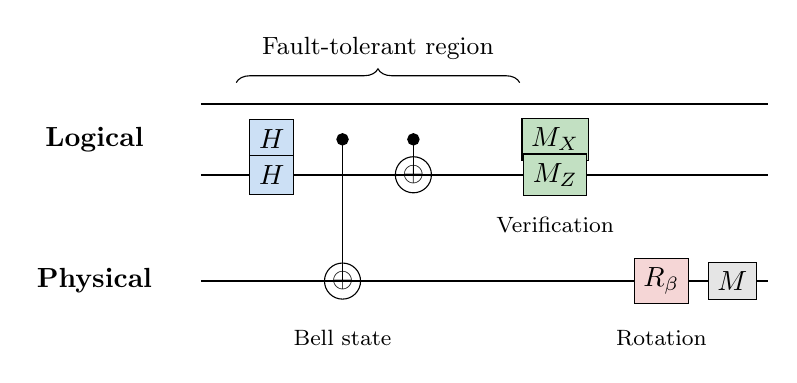
\begin{tikzpicture}[scale=0.9]
% Circuit diagram for hybrid verification
\node at (-1.5, 2) {\textbf{Logical}};
\node at (-1.5, 0) {\textbf{Physical}};

% Logical qubits (encoded)
\foreach \y in {1.5, 2.5} {
    \draw[thick] (0,\y) -- (8,\y);
}

% Physical qubit
\draw[thick] (0,0) -- (8,0);

% Gates - encoding
\node[draw, fill=quantumblue!20, minimum size=0.5cm] at (1, 2) {$H$};
\node[draw, fill=quantumblue!20, minimum size=0.5cm] at (1, 1.5) {$H$};

% Bell pair preparation
\draw[fill=black] (2,2) circle (0.08);
\draw (2,2) -- (2,0);
\node[draw, circle, inner sep=1pt] at (2,0) {$\oplus$};

% Entangling gates
\draw[fill=black] (3,2) circle (0.08);
\draw (3,2) -- (3,1.5);
\node[draw, circle, inner sep=1pt] at (3,1.5) {$\oplus$};

% Verification measurements
\node[draw, fill=hybridgreen!30] at (5, 2) {$M_X$};
\node[draw, fill=hybridgreen!30] at (5, 1.5) {$M_Z$};

% Physical operation
\node[draw, fill=classicalred!20, minimum size=0.5cm] at (6.5, 0) {$R_\beta$};

% Final measurement
\node[draw, fill=gray!20] at (7.5, 0) {$M$};

% Labels
\node[font=\footnotesize] at (2, -0.8) {Bell state};
\node[font=\footnotesize] at (5, 0.8) {Verification};
\node[font=\footnotesize] at (6.5, -0.8) {Rotation};

% Brace for encoded region
\draw[decorate, decoration={brace, amplitude=5pt}] (0.5, 2.8) -- (4.5, 2.8) node[midway, above=5pt, font=\small] {Fault-tolerant region};

\end{tikzpicture}
\caption{Hybrid verification circuit combining fault-tolerant logical operations with physical rotations, following \cite{majidy2025scalable}.}
\label{fig:hybrid}
\end{figure}

\textbf{Noise Model:} We adopt the depolarizing channel model from \cite{majidy2025scalable} with error rates $p_0$ (idle), $p_1$ (single-qubit), $p_2$ (two-qubit), and $p_3$ (measurement).

\section{Expected Contributions}

\begin{enumerate}
    \item \textbf{Theoretical:} Formal characterization of k-uniformity in random cluster states, establishing conditions under which MBQC verification inherits fault tolerance from k-uniform state preparation.
    
    \item \textbf{Algorithmic:} Adaptive verification protocols (Algorithm~\ref{alg:adaptive}) with provable sample complexity bounds exploiting k-uniform structure.
    
    \item \textbf{Practical:} Noise-aware verification thresholds for near-term experiments targeting quantum advantage with $\mathcal{O}(50 \times 50)$ cluster states \cite{ringbauer2025verifiable}.
\end{enumerate}

\textbf{Value Proposition:} This research enables the first fault-tolerant verification of quantum random sampling, addressing a key bottleneck identified in \cite{ringbauer2025verifiable}: ``Our results and techniques provide a feasible path toward a verified demonstration of quantum advantage.'' By integrating the k-uniform framework from \cite{majidy2025scalable}, we extend this path to include error protection during verification itself.

\section{Conclusion}

This proposal addresses the critical gap between MBQC verification protocols and fault-tolerant k-uniform state preparation. By establishing theoretical connections through stabilizer formalism and developing adaptive algorithms, we aim to enable verified quantum advantage demonstrations on near-term devices. The research directly addresses foundational questions about quantum-classical computational boundaries while providing practical tools for experimental implementation.

The proposed work builds naturally on Prof. Hangleiter's contributions to quantum random sampling verification \cite{ringbauer2025verifiable} and k-uniform state theory \cite{majidy2025scalable}, while leveraging my background in optimization algorithms and machine learning for efficient protocol design. I am committed to rigorous theoretical analysis combined with attention to experimental feasibility, following the research philosophy demonstrated in Prof. Hangleiter's work.

\bibliographystyle{IEEEtran}
\begin{thebibliography}{10}

\bibitem{ringbauer2025verifiable}
M. Ringbauer, M. Hinsche, T. Feldker, P. K. Faehrmann, J. Bermejo-Vega, C. L. Edmunds, L. Postler, R. Stricker, C. D. Marciniak, M. Meth, I. Pogorelov, R. Blatt, P. Schindler, J. Eisert, T. Monz, and D. Hangleiter, ``Verifiable measurement-based quantum random sampling with trapped ions,'' \emph{Nature Communications}, vol. 16, p. 106, 2025.

\bibitem{majidy2025scalable}
S. Majidy, D. Hangleiter, and M. J. Gullans, ``Scalable and fault-tolerant preparation of encoded k-uniform states,'' \emph{arXiv preprint arXiv:2503.14506}, 2025.

\bibitem{bluvstein2024logical}
D. Bluvstein, S. J. Evered, A. A. Geim, S. H. Li, H. Zhou, T. Manovitz, S. Ebadi, M. Cain, M. Kalinowski, D. Hangleiter, \emph{et al.}, ``Logical quantum processor based on reconfigurable atom arrays,'' \emph{Nature}, vol. 626, pp. 58--65, 2024.

\bibitem{acharya2024quantum}
R. Acharya \emph{et al.}, ``Quantum error correction below the surface code threshold,'' \emph{arXiv preprint arXiv:2408.13687}, 2024.

\bibitem{ryananderson2024highfidelity}
C. Ryan-Anderson, N. Brown, C. Baldwin, J. Dreiling, C. Foltz, J. Gaebler, T. Gatterman, N. Hewitt, C. Holliman, C. Horst, \emph{et al.}, ``High-fidelity and fault-tolerant teleportation of a logical qubit using transversal gates and lattice surgery on a trapped-ion quantum computer,'' \emph{Science}, vol. 385, pp. 1327--1332, 2024.

\bibitem{dasilva2024demonstration}
M. P. Da Silva, C. Ryan-Anderson, J. M. Bello-Rivas, A. Chernoguzov, J. Dreiling, C. Foltz, J. Gaebler, T. Gatterman, D. Hayes, N. Hewitt, \emph{et al.}, ``Demonstration of logical qubits and repeated error correction with better-than-physical error rates,'' \emph{arXiv preprint arXiv:2404.02280}, 2024.

\bibitem{gidney2024cultivation}
C. Gidney, N. Shutty, and C. Jones, ``Magic state cultivation: Growing T states as cheap as CNOT gates,'' \emph{arXiv preprint arXiv:2409.17595}, 2024.

\bibitem{reichardt2024demonstration}
B. W. Reichardt, A. Paetznick, D. Aasen, I. Basov, J. M. Bello-Rivas, P. Bonderson, R. Chao, W. van Dam, M. B. Hastings, A. Paz, \emph{et al.}, ``Demonstration of fault-tolerant Steane quantum error correction,'' \emph{arXiv preprint arXiv:2411.11822}, 2024.

\bibitem{hong2024entangling}
Y. Hong, E. Durso-Sabina, D. Hayes, and A. Lucas, ``Entangling four logical qubits beyond break-even in a nonlocal code,'' \emph{Physical Review Letters}, vol. 133, p. 180601, 2024.

\bibitem{rodriguez2024experimental}
P. S. Rodriguez, J. M. Robinson, P. N. Jepsen, Z. He, C. Duckering, C. Zhao, K.-H. Wu, J. Campo, K. Bagnall, M. Kwon, \emph{et al.}, ``Experimental demonstration of logical magic state distillation,'' \emph{arXiv preprint arXiv:2412.15165}, 2024.

\end{thebibliography}

\end{document}
